\section{Overview and motivating example}
\label{sec:motivation}

In this section, we shall provide the motivation for our paper, an overview of our technique, and illustrate the method on a motivating example.

\subsection{Motivation: frame reasoning, delta changes and verification conditions}
In this part we shall describe the need for a new logic for expressing verification conditions for Hoare triples involving snippets of code that modify a bounded set of heap locations.

Let us consider a set of pointer fields $\vect{p}$ and a recursive definition of a unary predicate or function $R(x)$ defined
using least fixpoints over $\vect{p}$. Typical functions include properties such as 
``$x$ points to a linked list segment ending at the location $z$'', ``the length of the list pointed to by $x$'', 
``$x$ points to a binary search tree'', ``the set of keys stored in the tree pointed to by $x$'', ``the heaplet defined
by the tree pointed to by $x$'', etc.
Consider a Hoare triple of the form $\textit{@pre}(\vect{x}, \vect{p}, R) ~S~ \textit{@post}(\vect{x}, \vect{p}, R)$; the pre and postconditions use the recursively defined predicate/function $R$.

One simple approach is to capture the precondition using logic and use the \emph{frame rule} to reason soundly
(but incompletely) about the post-state--- i.e., we can simply ignore the definition of $R$
on the transformed heap and infer that $R(x)$ holds in the post-state if it held in the pre-state and 
the modified portion of the heap did not intersect with the underlying heaplet of $R(x)$.
This is, in practice, a very \emph{convenient and simple} reasoning that often works and is one of the foundational ideas that separation logic facilitates~\cite{Reynolds2002}. However, vanilla frame reasoning can be incomplete, as we shall argue through a motivating example (see Section~\ref{sec:motivating_example}). 

The focus of this paper is on the generation of precise verification conditions for basic blocks that do not involve function calls. For basic blocks that involve function calls, our recommendation is to use frame reasoning, \emph{\`a la} separation logic. 

Let us now consider basic blocks that do not involve function calls. We would like
to generate precise verification conditions in such cases. There are several approaches in the literature that argue for this: for example the Grasshopper suite of tools
handle such blocks accurately for certain logics~\cite{PiskacWiesZufferey2014}, and there is work on expressing weakest preconditions in separation logic for such blocks using the magic wand~\cite{Reynolds2002}; see section on related work. The goal of this paper is to accurately formulate verification conditions for very expressive logics (FO+\textit{lfp}) that can also be reasoned with effectively, especially in the context of decidable logics.

One precise formulation of the verification condition is of the form:
$$\left(\textit{@pre}(\vect{x}, \vect{p}, R) \wedge\, T(\vect{x}, \vect{x}', \vect{p}, \vect{p}')\right) \Rightarrow\, \textit{@post}(\vect{x}', \vect{p}', R')$$
where $T$ describes the effect of the program on the stack and the heap, describing how the scalar variables $\vect{x}$ and pointer-fields $\vect{p}$ have evolved to the $\vect{x}'$ and $\vect{p}'$ respectively. Most importantly, the above requires \emph{new} recursive definitions $R'$ that are formulated by replacing $\vect{p}$ in the definition of $R$ with $\vect{p}'$. 

Though the above is a precise formulation of the verification condition, it has several drawbacks. First, there is a heaplet $H$
modified by the program, and the formula will have conjuncts of the form $\forall y \not \in H. p'(y)=p(y)$, for every $p \in \vect{p}$. This introduces
universal quantification, which is harder to reason with automatically. However, for basic blocks that do not involve
function calls, $H$ is finite, and we can map this into a decidable quantifier-free logic (modeling $p$ as an array
and $p'$ as an update to the array).
Second, the new definition of $R'$ depends on $\vect{p}'$, which in turn depends on the various constraints introduced by the basic
block. For example, pointer fields may change depending on complex properties involving the data elements stored in the heap.
Reasoning with $R'$ automatically (which involves least fixpoints), coupled with such constraints, is daunting.

\emph{Surely, there must be a simpler formulation of the verification condition!} Small changes to the heap do cause global changes and
can dramatically affect the valuation of recursively defined predicates/functions, which are global.
But surely, the effect on the semantics of $R$ changing into $R'$ must be expressible in a simpler localized fashion.

The goal of this paper is to identify such a logic.


\subsection{Overview of method}

\paragraph{Delta-logics:}
In this paper, we describe a class of logics, called \emph{delta-logics}, that are logics for writing verification conditions of basic blocks without function calls and are precisely meant to address the issues mentioned in the above section. In particular, formulations in delta-logics will avoid the need for \emph{two} diferent recursive definitions $R$ and $R'$.
Instead, both $R$ and $R'$ will be expressed as the same recursive definition, but parameterized using different sets of first-order variables
(as opposed to being parameterized over two different sets of first-order \emph{functions}, $\vect{p}$ and $\vect{p'}$ as above).

Formulae in delta-logics are Boolean combinations of two distinct kinds of formulae: one kind, called \emph{delta-specific} formulae, strictly talk about the modified portion of the global heap (identified by a bounded set of locations $\Delta$) without using
any recursive definitions; the other 
kind, called \emph{contextual} formulae, strictly talk about the unbounded portion excluding $\Delta$ using recursive definitions (see Figure~1).
A set of first-order interface variables are used to communicate information between $\Delta$ and the rest of the heap (its `context'). In particular, a recursive definition $R$ over the unbounded context is \emph{parameterized}
over a set of first-order communication variables $P^R$, where $P^R$ summarizes the values of $R$ within $\Delta$. These variables themselves can, of course, depend on the value of $R$ outside $\Delta$ as well, setting up mutually dependent constraints. 

\begin{figure}
  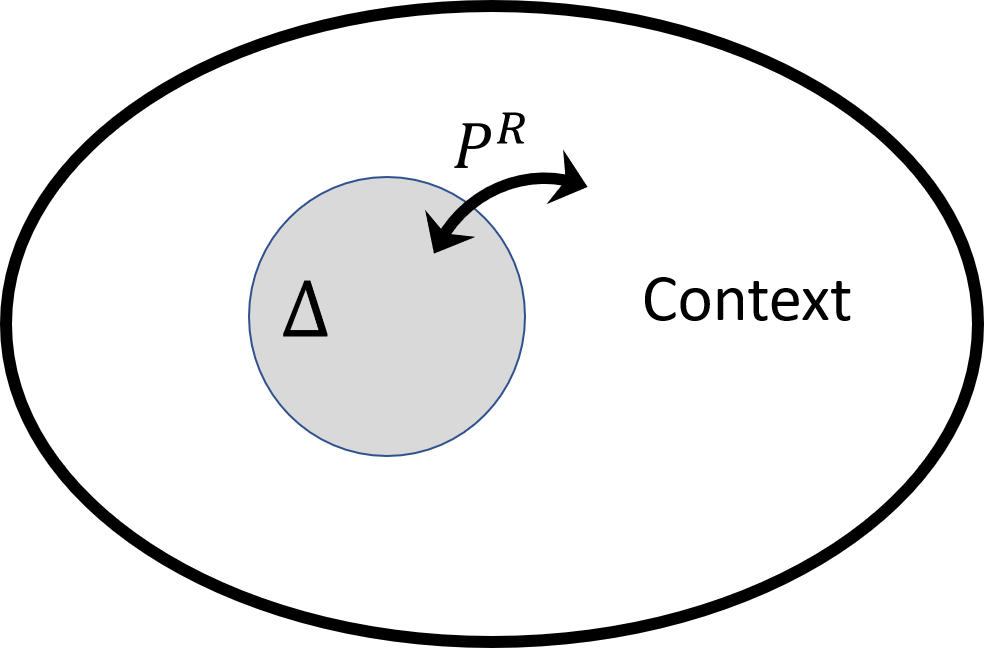
\includegraphics[width= 50mm]{PR.png}
  \caption{Delta-logic}
  \label{pr}
\end{figure}


\paragraph{Advantages of reasoning with Delta-logics:}
Expressing verification conditions in delta-logics has a distinct advantage in automated reasoning. We formulate verification conditions in delta logics in the following manner (see Figure~\ref{blobs}).
We can view the program's transformation of pre-heap to the post-heap as a static model consisting of three different submodels: one is the context heap, the second is the pre-heap restricted to $\Delta$, and the third is the post-heap restricted to  $\Delta$.
Note that there is only one context heap as it does not change, and this context heap is infinite, in general. However, the other two heaps are finite. The recursive properties of the heap are then defined  on the context-heap, parameterized with the communication variables $P_R$ for expressing properties of the pre-heap, and parameterized over the communication variables $P_R'$ for expressing properties of the post-heap.

The key advantage of the above model is that
two of the submodels (both over $\Delta$) are finite, and reasoning about them and the data-fields accessible from them can be automated using standard SMT solvers.
The context heap is the single unbounded submodel that poses automation challenges. In this paper, we exploit this simplicity of dealing only with one infinite submodel (as opposed to the naive formulation, which would have two infinite submodels) to build new powerful classes of decidable logics over lists and list-measures. 

\begin{figure}
  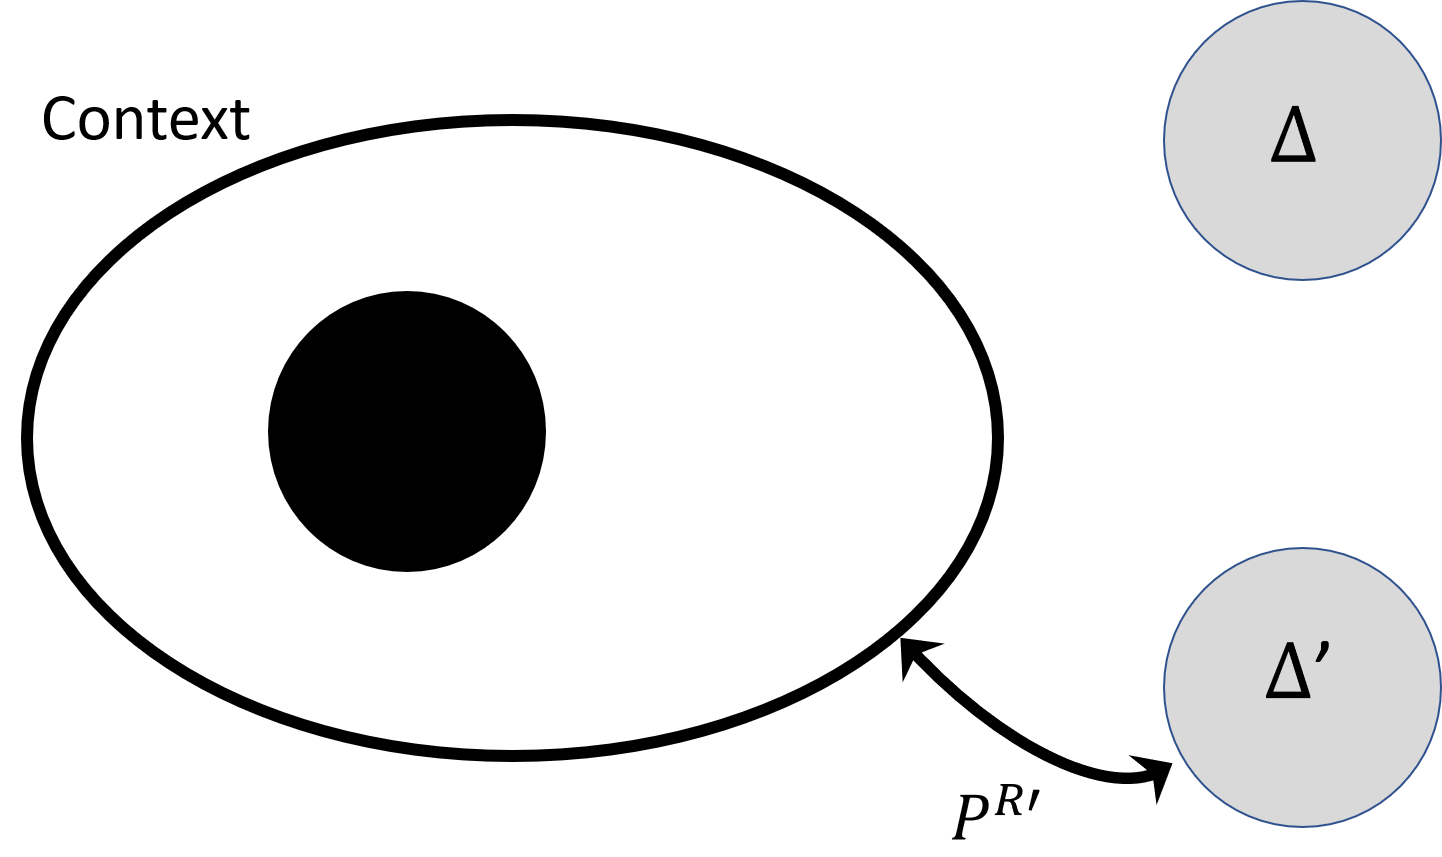
\includegraphics[width= 50mm]{3blobs.png}
  \caption{VC expressed in delta-logics}
  \label{blobs}
\end{figure}


\paragraph{Expressing verification conditions in Delta-logics}
With the above model of verification conditions in mind, let us examine how to write VCs corresponding to Hoare triples in delta-logics. The key idea is to set up parameterized sets of recursive definitions with two sets of parameters $P_R$ and $P_R'$, as described above, expressing the precondition using
one and the postcondition using the other. The program transformation of the $\Delta{}$ portion of the pre-heap to that of the post-heap can be described in quantifier-free FO,  since they are finite.

The main challenge that remains is to express the precondition and postcondition using Delta logics.
%, and the pre- and post-conditions can be translated to delta-logic formulae using the separability theorem. Notice that this captures naturally the changing $\Delta$ portion of the heap while keeping the context unchanged and 
%hence removes the need for the universally quantified formula asserting that pointers in the context have not changed.
In order to do this, we prove a general technical result for delta-logics, called the \emph{separability theorem} in Section~\ref{sec:separability}. This theorem shows that any quantifier-free FO formula
with recursive definitions (with \textit{lfp} semantics) can be expressed in delta-logics: as a boolean combination of delta-specific formulae
and contextual formulae. 

The separation theorem sets up communication between the two portions: the $\Delta$ portion of the heap 
and its context. The context is handled using the parameterized recursive definitions and the $\Delta{}$ portion, being finite, is handled by `unfolding' the recursive definition across $\Delta{}$. This unfolding would stop at the `boundary' of $\Delta{}$ and the context, which is where we use the interface variables to communicate the valuations across these disjoint portions. These are the mutual constraints that were referred to earlier in this section.
However, it turns out that a new set of recursive definitions and communication variables involving a notion of \emph{rank} for each (parameterized) recursive definition is
needed to accurately capture least fixpoints, for the parameterized recursive functions are now merely defined on the context and the \textit{lfp} semantics cannot be preserved by a naive unfolding of the definition, even if the portion on which the unfolding is done is finite (for instance, the familiar definition of lists as either being $nil$ or pointing to a location that points to a list is incorrect with just fixpoint semantics, as it would then be acceptable to call a cycle a list as well). These ranks can, however, be constrained to be \emph{bounded integers} as opposed to ordinals (though the heap is infinite). 


\paragraph{Decidable Delta-logics}
  As a culmination of the above arguments, we demonstrate the efficacy of delta-logics to build a powerful program logic for reasoning with manipulations of lists and list-measures. The decision procedure crucially relies on the simplicity of VCs expressed in delta-logics--- having \emph{one} infinite contextual heap, two finite heaplets and communication between them using only first-order variables.


\subsection{Motivating Example}
\label{sec:motivating_example}
We shall now illustrate our method on a motivating example.
Let us consider the following Hoare triple with pre/post conditions written in FO+\textit{lfp}:\\
\centerline{$ \{ list(x) \wedge  list(w) \wedge  y \not \in hlist(w) \} 
~~~~~\texttt{y.next := w}~~~~~
\{list(x) \}$}\\
where $list(x)$ is a recursive definition that that holds when $x$ points to a list, and in which
case, $hlist(x)$, another recursive definition, captures the set of locations in that list. We omit these definitions.

It is easy to see that this Hoare Triple is valid. First notice that frame reasoning argues that $w$ continues to point to a list.
There are then two cases: if $y$ does not belong to the list pointed to by $x$, then since $y$ is not in the heaplet, frame reasoning would prove that $x$ continues to point to a list.
However, in the case when $y$ does belong to the list pointed to by $x$, we cannot use frame reasoning to immediately conclude that $x$ will continue to point to a list. However, notice that $x$ will point to a list in this case as well, since $y$ will point to $w$ which points to a list. Therefore, frame reasoning \emph{alone} will not be sufficient to conclude the postcondition from the precondition and the program transformation at this point. 

The naive VC for this program is expressed by using a new $next$ pointer (say, $next'$) to model the post-state of the program, redefining the recursive functions and predicates using $next'$ to talk about valuations on the post-state, and observing that $next$ has not changed on any other location except for that pointed to by $y$:

\begin{center}
$\Big( \big( list(x) \wedge  list(w) \wedge  y \not \in hlist(w) \big) \land{} \big( \left(next'(y) = w \land{} y' = y \land{} w' = w \land{} x' = x\right) \land{} \left(\; \forall{}u.\, u\neq{}y \Rightarrow{} next'(u) = next(u)\; \right) \big) \Big) \Rightarrow{} \left(list'(x')\right)$
\end{center}
where the quantifier is interpreted to range over all locations on the heap. We shall now convert this to a VC in delta-logic.

In this case, the set of modified locations is $\Delta{} = \{y\}$. To write the VC in delta-logic we shall first use the separability theorem (Section~\ref{sec:separability}) to write the pre- and and post-conditions in delta-logic. The separability theorem introduces new parameterized \emph{rank} functions for each parameterized recursive definition. For the precondition, this yields a delta-logic formula of the kind:
\begin{center}
 $\left(list^{P}(x) \wedge  list^{P}(w) \wedge  y \not \in hlist^{P}(w)\right) ~~\land{}~~ \beta{}(P)$
\end{center}
where $list^{P}()$ and $hlist^{P}()$ are the parameterized versions with the parameter set $P$. The domain of all of these definitions is the context, and therefore the formula $\left(list^{P}(x) \wedge  list^{P}(w) \wedge  y \not \in hlist^{P}(w)\right)$ is a contextual formula. $\beta{}$ is a delta-logic formula that accurately captures the least fixpoint semantics of the original definitions using the ranks and communication variables $P$. Similarly, we can also write the post-condition in delta-logic as $list'^{Q}(x') \land{} \beta{}(Q)$.

Substituting these into the VC gives:

\begin{center}
$\Big( \big( \left(list^{P}(x) \wedge  list^{P}(w) \wedge  y \not \in hlist^{P}(w) \right) \land{} \beta{}(P) \big) \land{} \big( \left(next'(y) = w \land{} y' = y \land{} w' = w \land{} x' = x\right) \land{} \left(\; \forall{}u.\, u\neq{}y \Rightarrow{} next'(u) = next(u)\; \right) \big) \Big) \Rightarrow{} \left(list'^{Q}(x') \land{} \beta{}(Q) \right)$
\end{center}

We now come to the crux of the versatility of delta-logics in expressing VCs. 
Notice that $list'^Q(x')$ on the
right of the implication above is a \emph{contextual} formula defined using $next'$. However, on the context, $next'$ is precisely $next$. Hence we can replace $list'^Q(x')$ with $list^Q(x')$, the latter being defined in terms of $next$. Since $next'$ is never used on the context, we can drop the universally quantified clause, giving us the VC:

\begin{center}
$\Big( \big( \left(list^{P}(x) \wedge  list^{P}(w) \wedge  y \not \in hlist^{P}(w) \right) \land{} \beta{}(P) \big) \land{} \big( \left(next'(y) = w \land{} y' = y \land{} w' = w \land{} x' = x\right) \big) \Big) \Rightarrow{} \left(list^{Q}(x') \land{} \beta{}(Q) \right)$
\end{center}
It is clear that this is a \emph{quantifier-free} delta-logic formula, and there is only one recursive definition for \emph{list} which is defined using $next$, though it is parameterized with $P$ and $Q$.
\medskip

The problem now reduces to solving for the validity of this VC in delta-logic. In the decidability section (Section~\ref{sec:decidability}), we show exactly how to build an effective procedure to decide the validity of delta-logic formulae over lists with various measures (which, in fact solve this particular example as well; see Section~\ref{sec:experiments}). The problem really is of finding a decision procedure for the solution of contextual formulae. To do this we observe that the context can be abstracted by a finite set of locations, and the list segments between them, if they exist, summarized in a way that can be encoded in SMT. We shall describe this in further detail in Section~\ref{sec:decidability}
